\newthought{\textbf{Zulfahmi - 2020903430056 - TRKJ 3B}}

\newday{\textbf{1 - 2 Desember 2022} - Instalasi dan Konfigurasi Hadoop}

\begin{enumerate}

\item Kendala dan Solusi
\begin{enumerate}
    \item kendala
\begin{itemize}
    \item Salah saat memasang ssh dengan memasukan password sehingga tidak dapat melanjutkan jobdesk selanjutnya
\end{itemize}
    \item solusi
\begin{itemize}
    \item Memasang kembali ssh tanpa menggunakan password
\end{itemize}
\end{enumerate}

\item Kesimpulan
\newline
    Pada Instalasi Apache Hadoop membutuhkan ruang yang
    cukup besar untuk mengekstrak file Apache Hadoop dan ram
    minimal 2gb agar bekerja optimal.


\begin{figure}[!ht]
    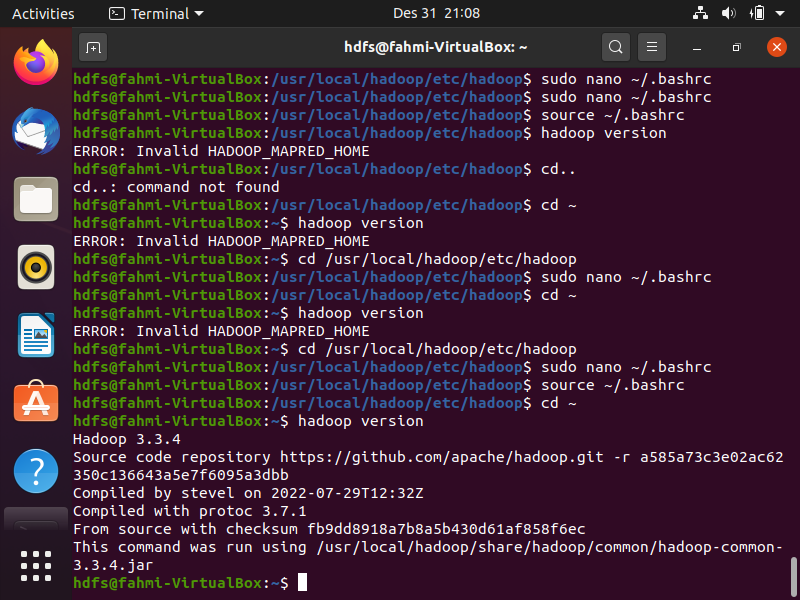
\includegraphics[width=\textwidth]{Zulfahmi/1. install apache hadoop}
    \caption{Install apache hadoop}
    \label{gam:Hasil}
\end{figure}

\begin{figure}[!ht]
    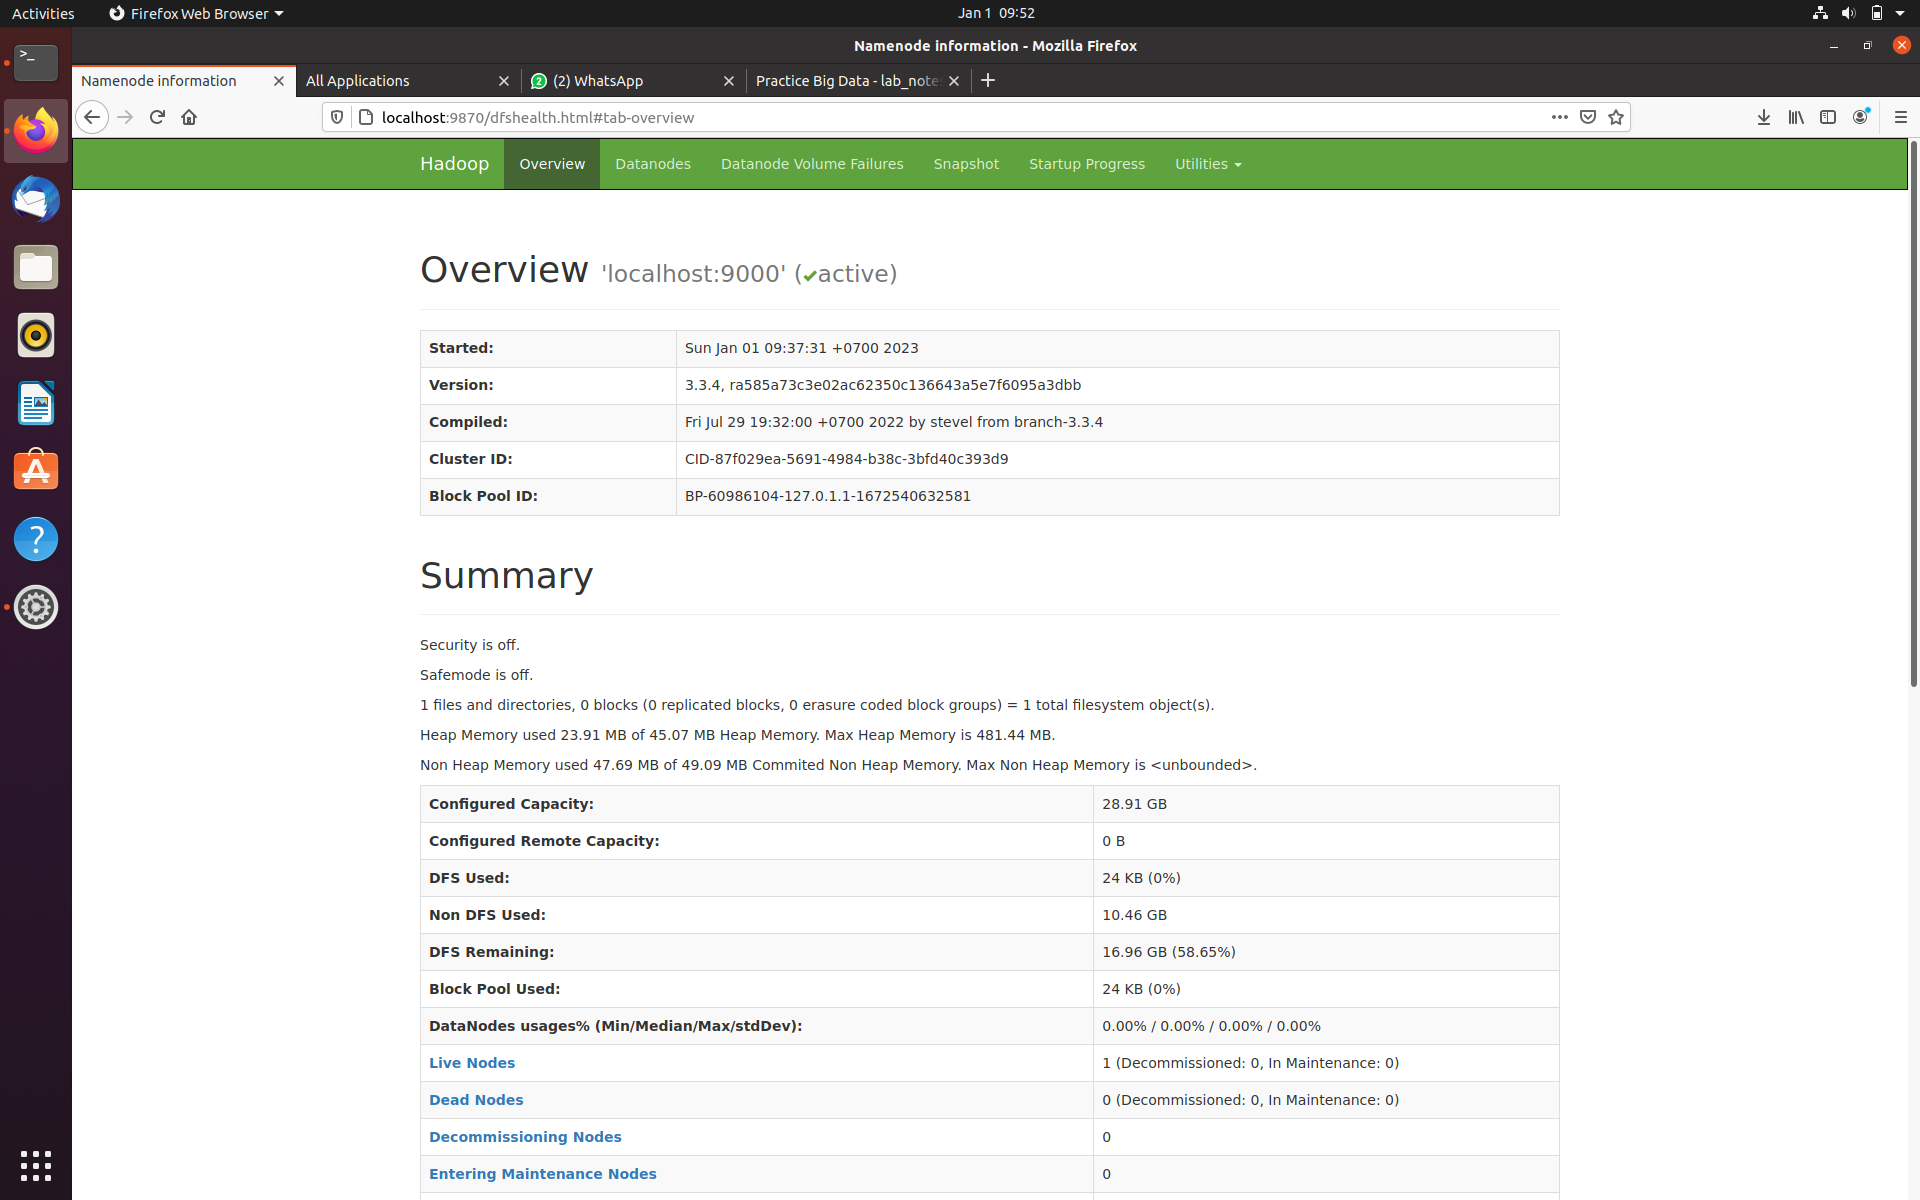
\includegraphics[width=\textwidth]{Zulfahmi/2. konfigurasi hadoop 1}
    \caption{konfigurasi hadoop}
    \label{gam:Hasil}
\end{figure}

\begin{figure}[!ht]
    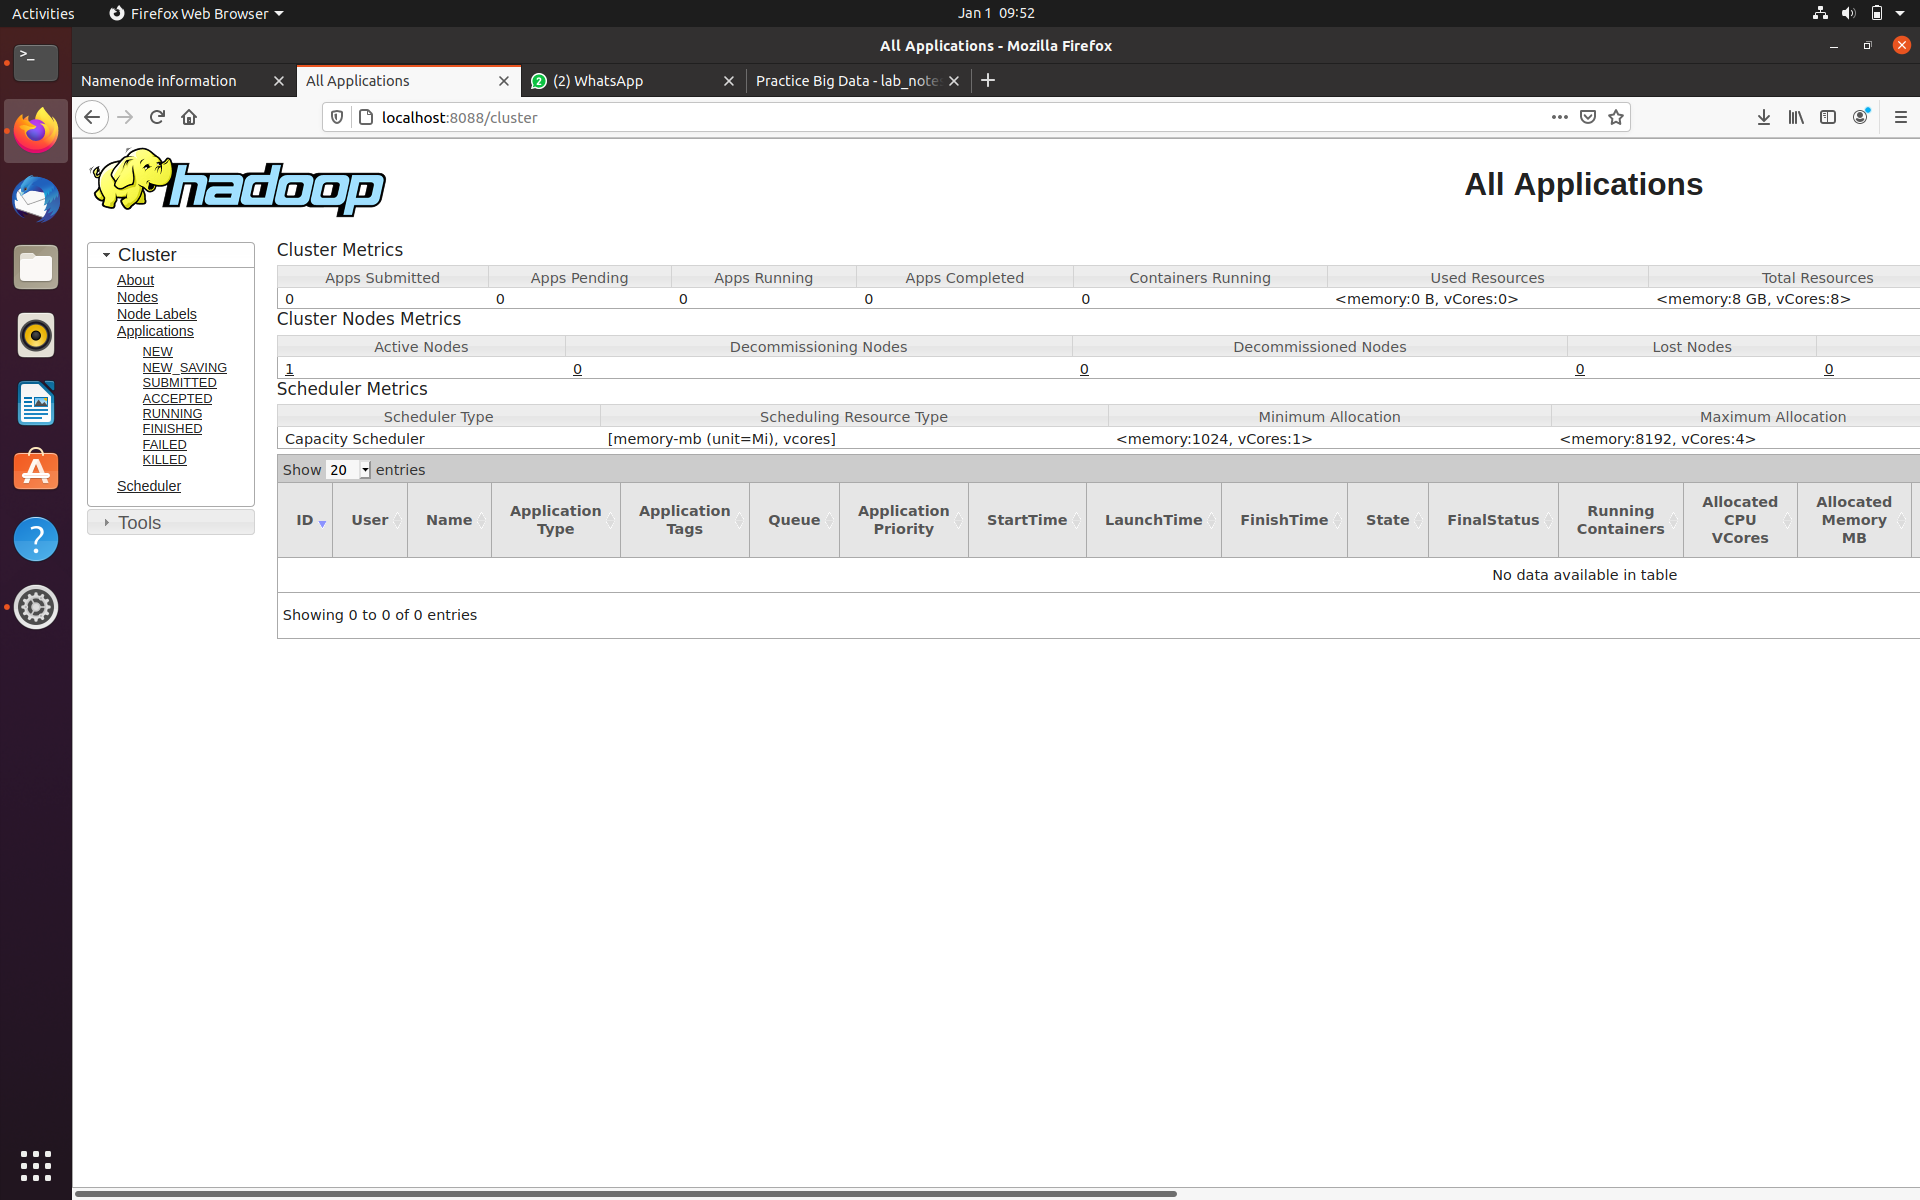
\includegraphics[width=\textwidth]{Zulfahmi/2. konfigurasi hadoop 2}
    \caption{konfigurasi hadoop}
    \label{gam:Hasil}
\end{figure}


\end{enumerate}

\clearpage
\newday{\textbf{8 Desember 2022} - WordCount bawaan Hadoop}
\begin{enumerate}
\item Kendala dan Solusi

\begin{itemize}
\item Tidak menemukan kendala apapun.
\end{itemize}

\item Kesimpulan
\newline
    Pada Hadoop terdapat program untuk menghitung jumlah kata 
    (WordCount) yang ada pada data. Sebagai praktikan melakukan input data terlebih
    dahulu, kemudian memprosesnya, sehingga menghasilkan data output.

\end{enumerate}

\begin{figure}[!ht]
    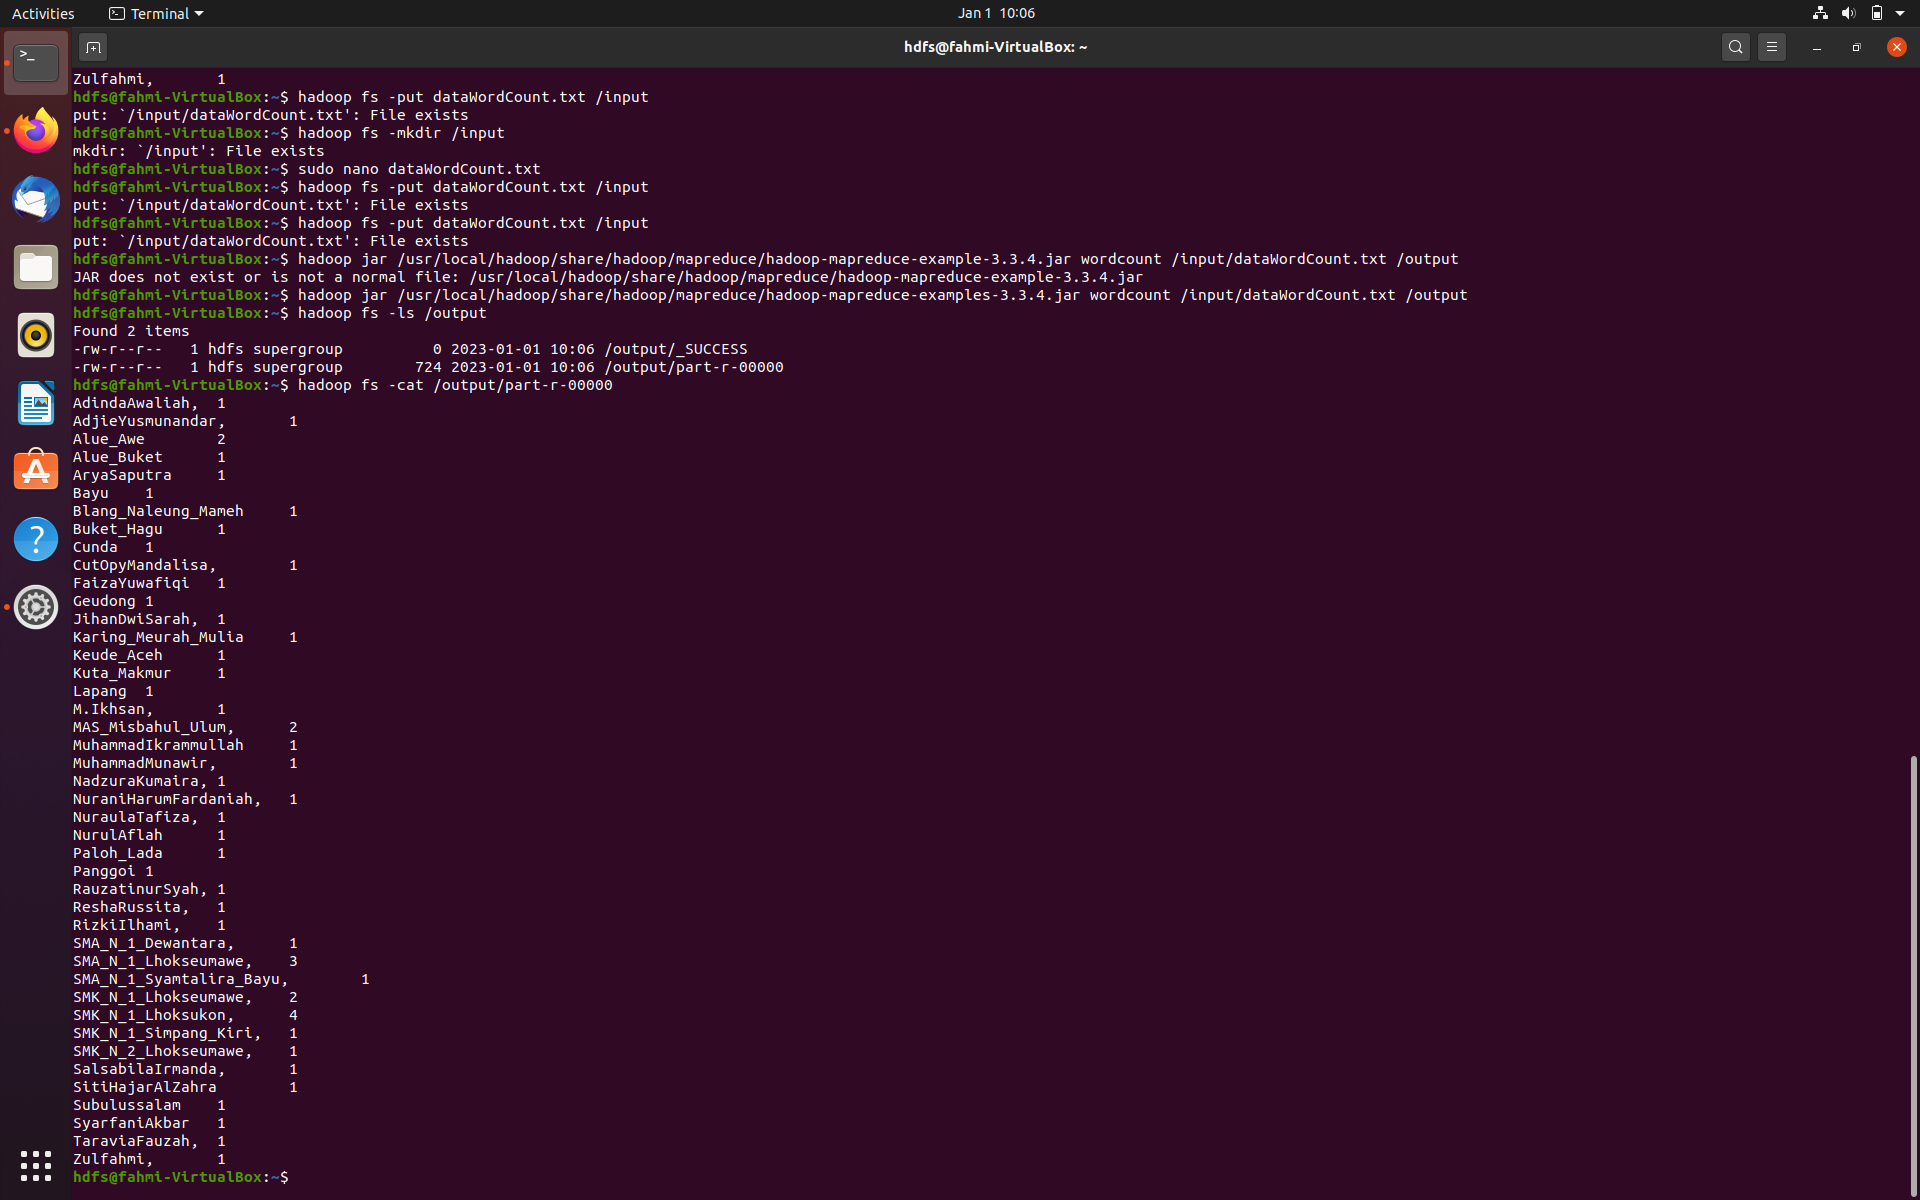
\includegraphics[width=\textwidth]{Zulfahmi/3. wordcount bawaan hadoop}
    \caption{hasil WordCount bawaan hadoop}
    \label{gam:Hasil}
\end{figure}

\clearpage
\newday{\textbf{9 Desember 2022} - WordCount dengan Java}
\begin{enumerate}
\item Kendala dan Solusi

\begin{itemize}
\item Tidak menemukan kendala apapun.
\end{itemize}

\item Kesimpulan
\newline
    Untuk hasil yang ditampikan sama dengan WordCount bawaan hadoop.

\end{enumerate}

\begin{figure}[!ht]
    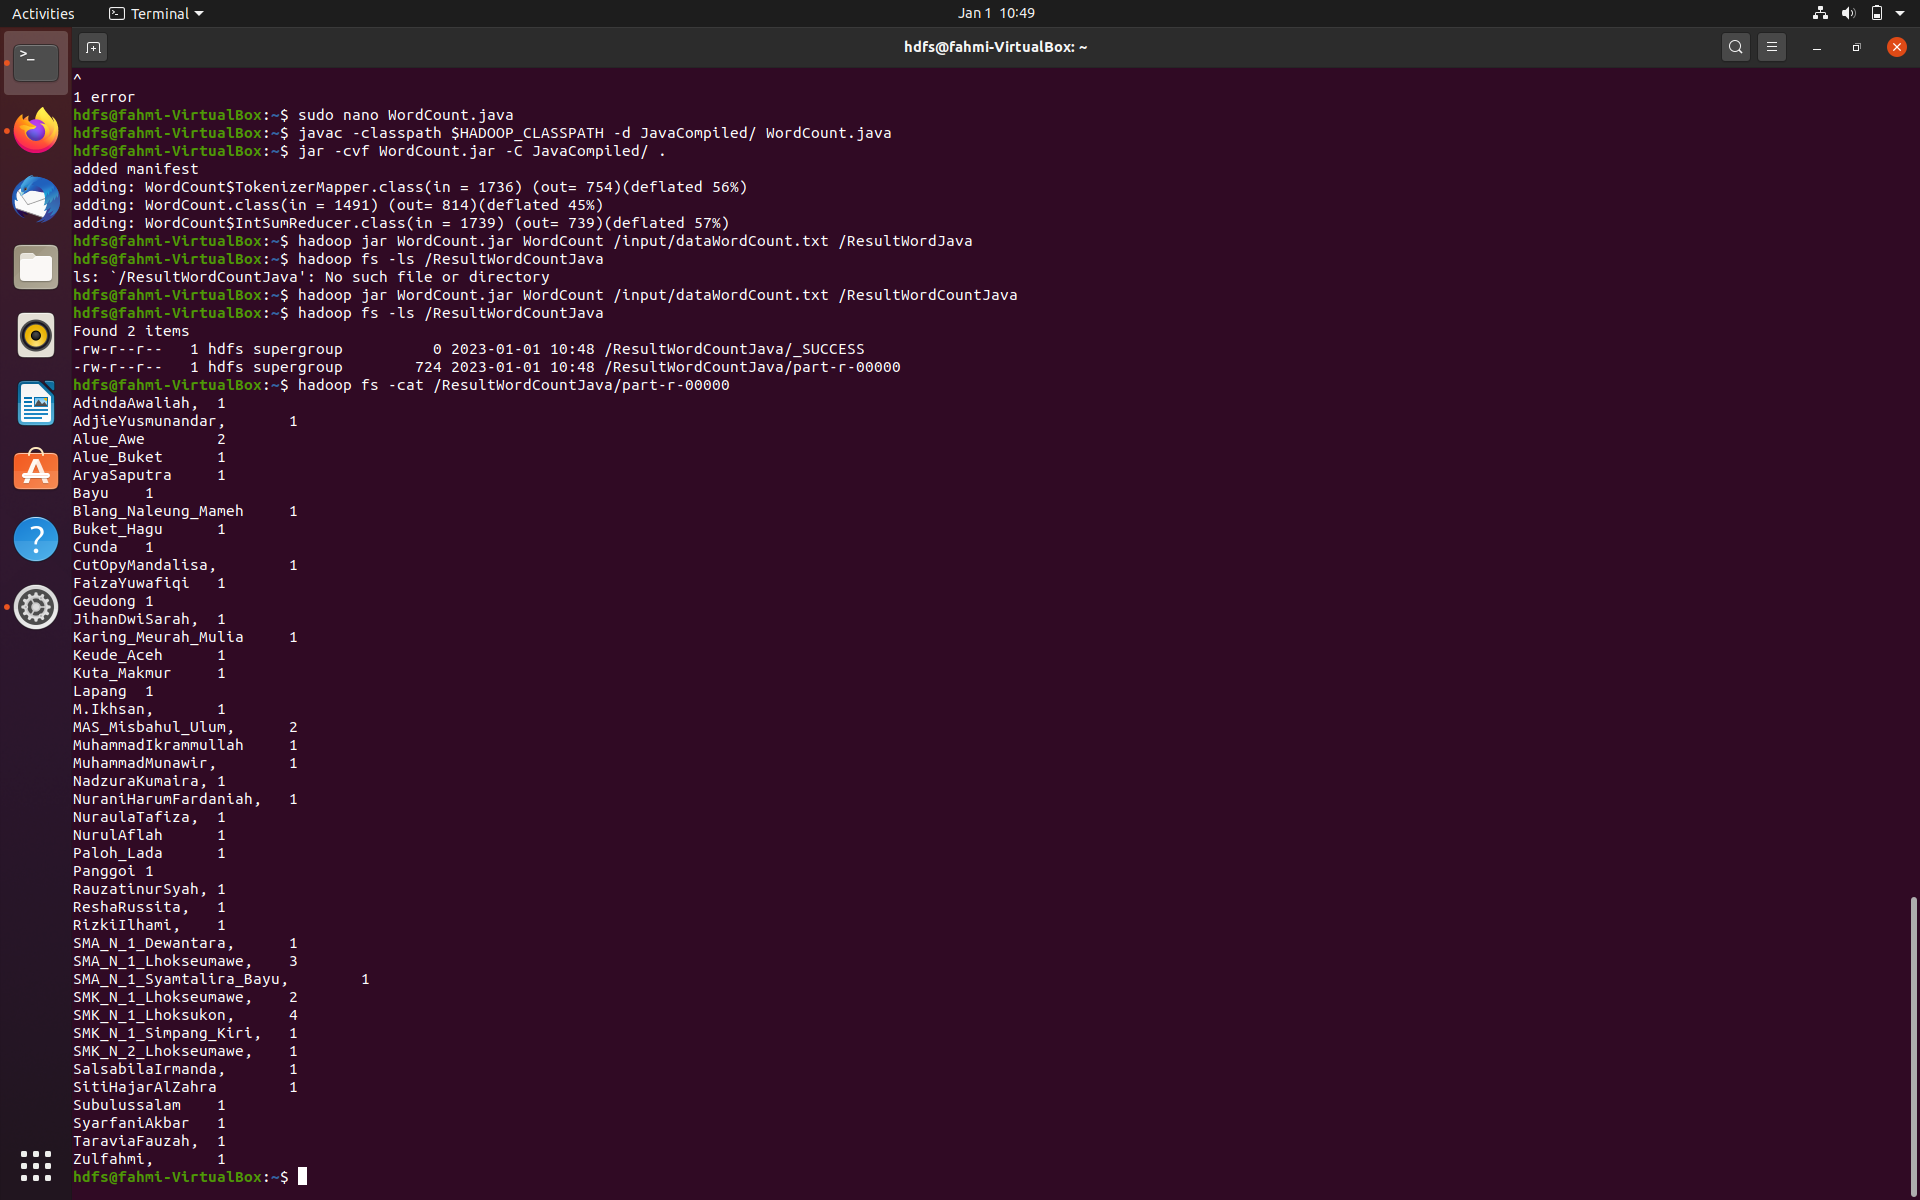
\includegraphics[width=\textwidth]{Zulfahmi/4. wordcount dgn java}
    \caption{hasil WordCount Java}
    \label{gam:Hasil}
\end{figure}


\clearpage
\newday{\textbf{15 Desember 2022} - Instalasi Apache Spark}
\begin{enumerate}
\item Kendala dan Solusi

\begin{itemize}
\item Tidak menemukan masalah apapun
\end{itemize}


\item Kesimpulan
\newline
    Apache Spark adalah sebuah framework komputasi
    yang dapat digunakan untuk mengakses data, memproses
    data, menanyakan data serta menganalisis big data

\end{enumerate}

\begin{figure}[!ht]
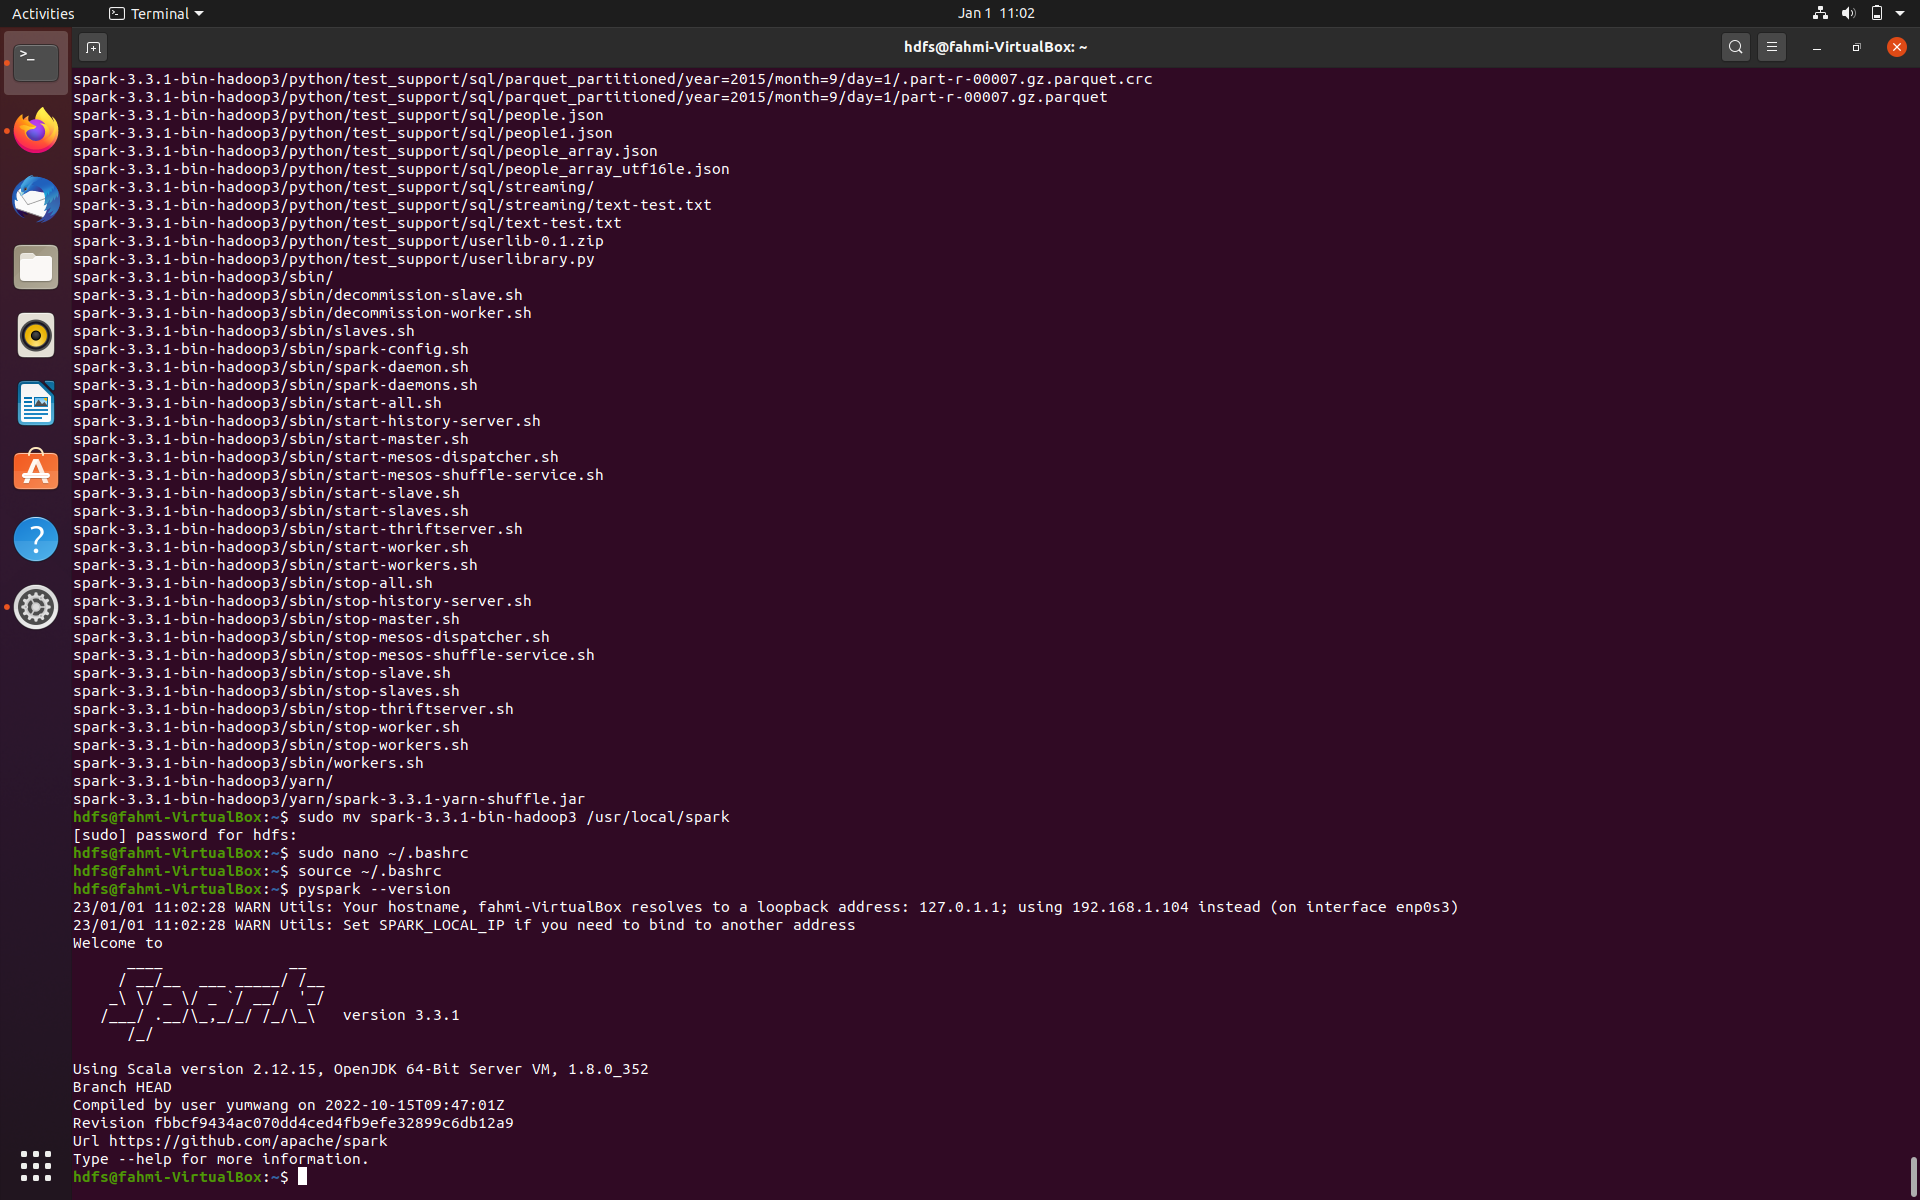
\includegraphics[width=\textwidth]{Zulfahmi/5. dw apache spark}
\caption{hasil instalasi apache spark }
\label{gam:hasil instalasi spark}
\end{figure}

\clearpage
\newday{\textbf{16 Desember 2022} - WordCount Dengan Python}
\begin{enumerate}
\item Kendala dan Solusi

\begin{itemize}
    \item Tidak menemukan kendala apapun.
\end{itemize}
    

\item Kesimpulan
\newline Berhasil menjalankan program WordCountPython dengan baik, walaupun banyak kendala yang dialami.


\begin{figure}[!ht]
    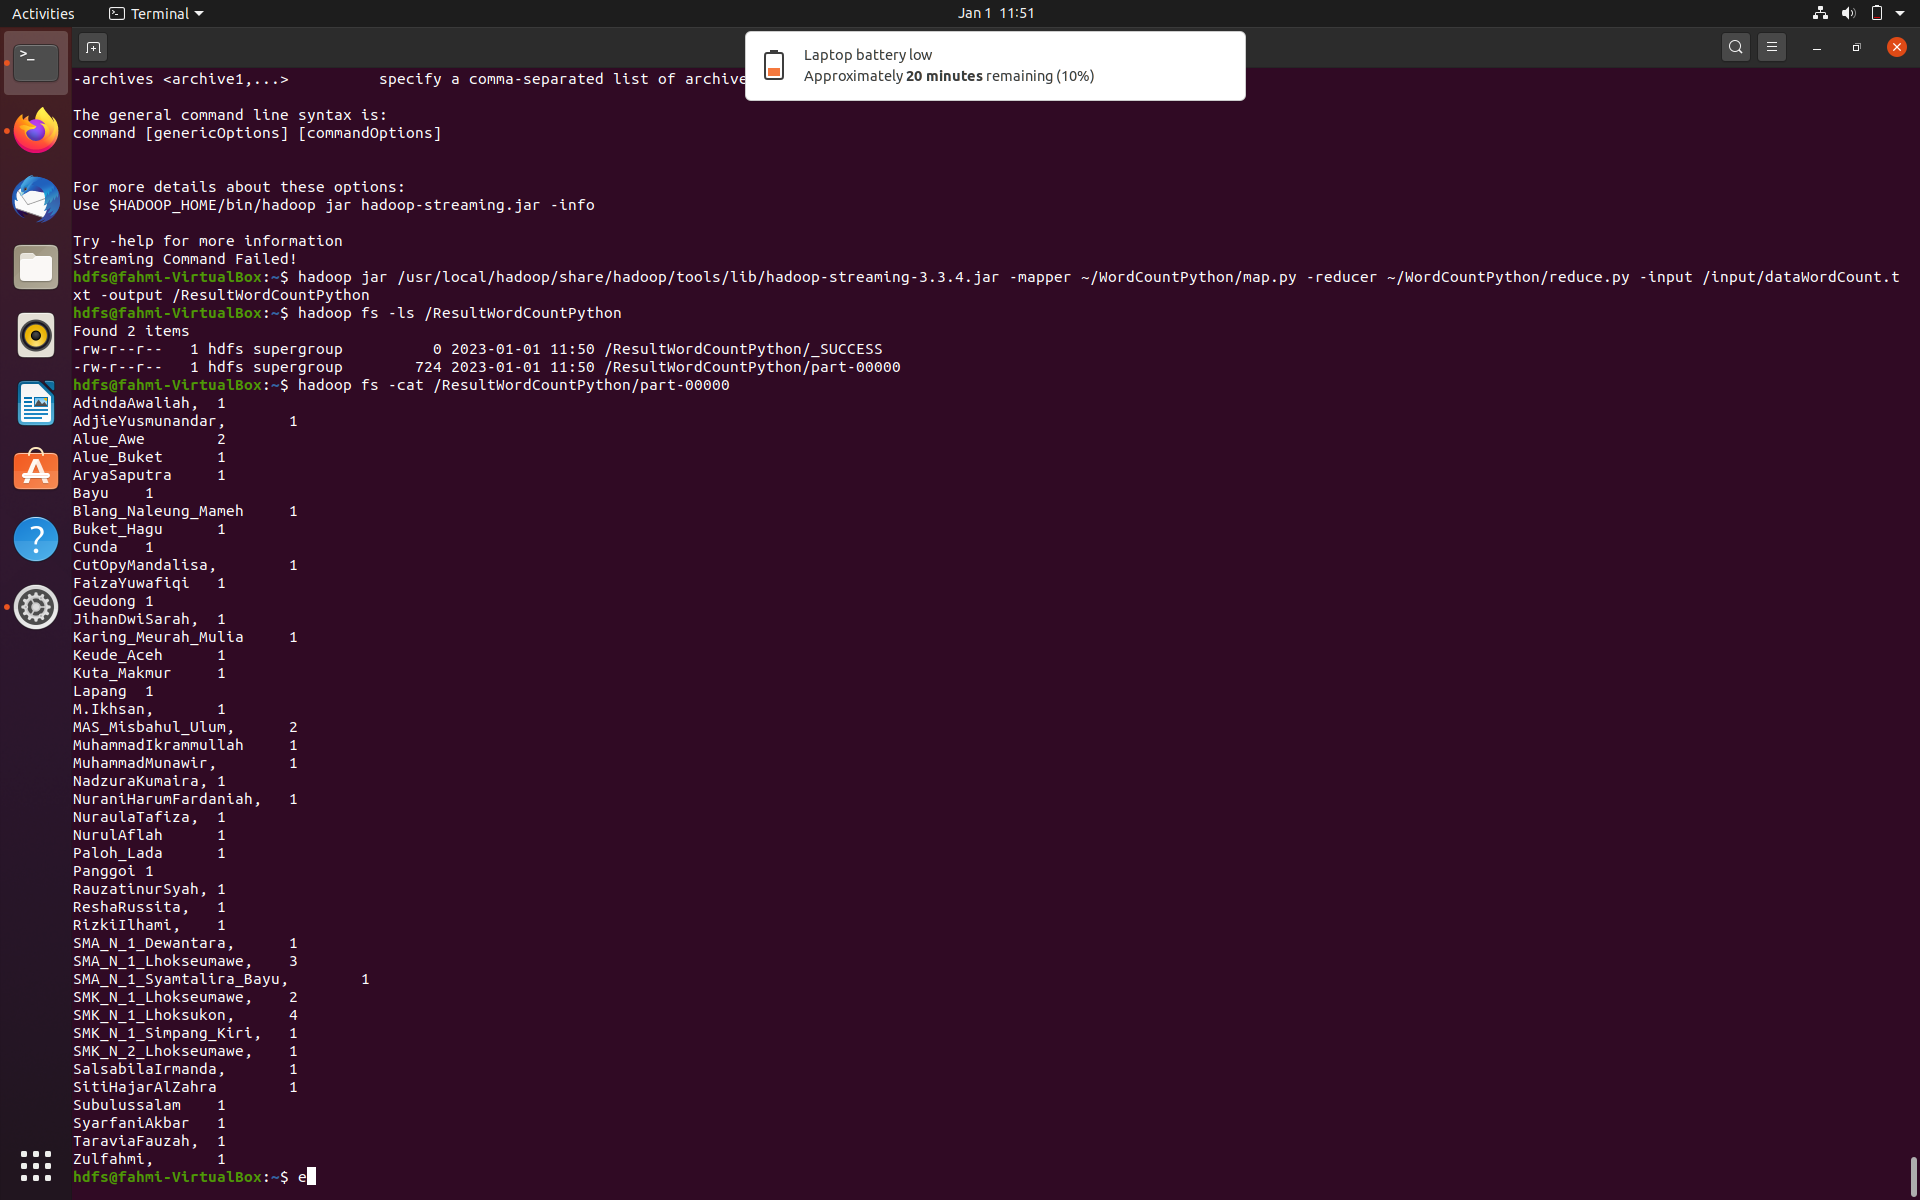
\includegraphics[width=\textwidth]{Zulfahmi/6. wordcount dgn python}
    \caption{wordcount dgn python}
    \label{gam:hasil WordCountPython}
    \end{figure}

\end{enumerate}

\clearpage
\newday{\textbf{22 Desember 2022} - WordCount dengan PySpark}
\begin{enumerate}
\item Kendala dan Solusi

\begin{itemize}
    \item Tidak menemukan kendala apapun.
\end{itemize}

\item Kesimpulan
\newline Program Berhasil berjalan walau ada sedikit kendala yang saya alami.

\end{enumerate}

\begin{figure}[!ht]
    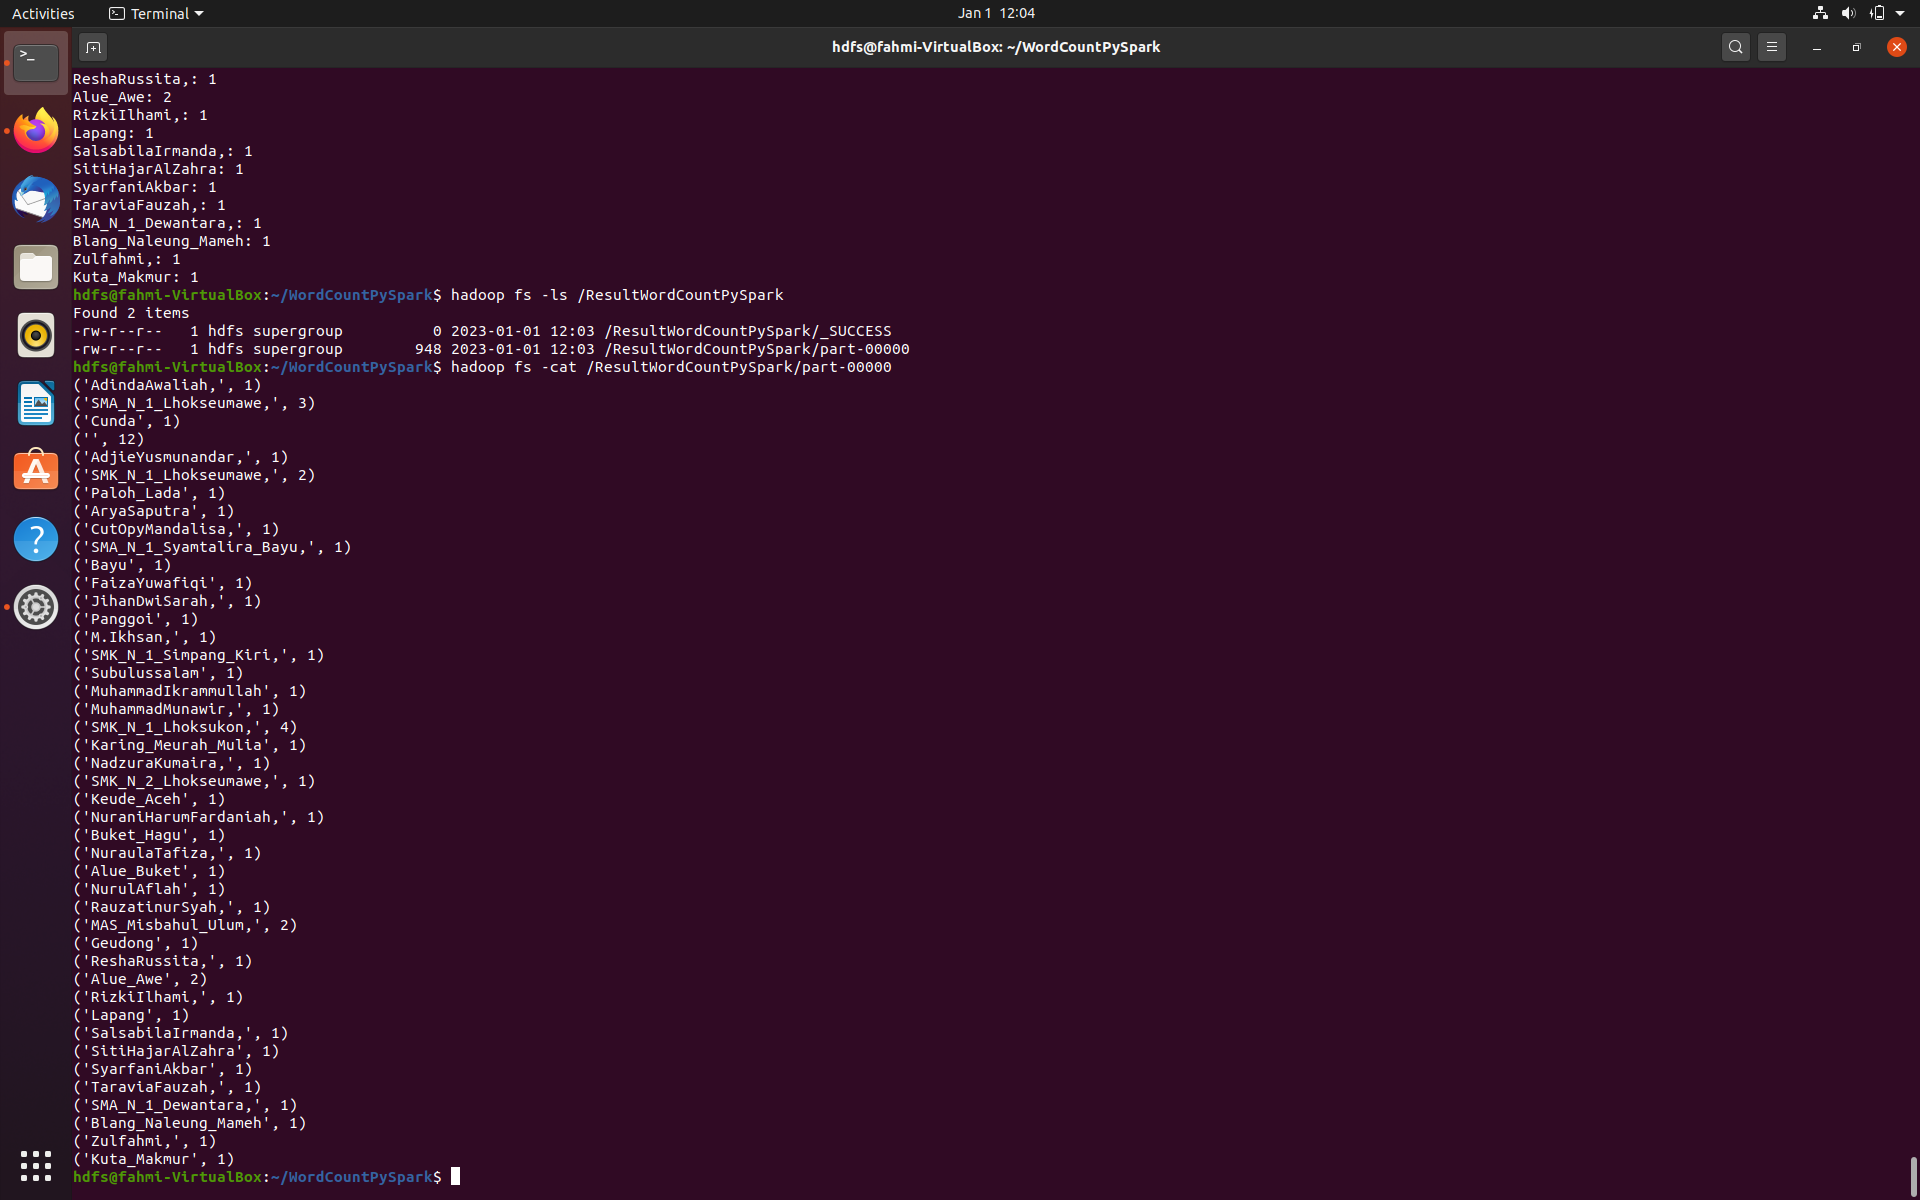
\includegraphics[width=\textwidth]{Zulfahmi/7. wordcount dgn pyspark}
    \caption{Hasil WordCount PySpark }
    \label{gam:hasil WordCountPyspark}
\end{figure}

\clearpage
\newday{\textbf{23 Desember 2022} - Machine Learning dengan PySpark}
\begin{enumerate}
\item Kendala dan Solusi

\begin{enumerate}
    \item kendala
\begin{itemize}
    \item Belum berhasil
\end{itemize}
    \item solusi
\begin{itemize}
    \item Terus mencoba
\end{itemize}
\end{enumerate}

\item Kesimpulan
\newline 

\end{enumerate}